\setcounter{page}{1}
\section*{Zielsetzung}
In dem Versuch $V408$ soll die Brennweite unterschiedlicher Linsen und
Linsensysteme untersucht werden.
\section{Theorie}
Für das betreiben von geometrischer Optik werden \emph{Linsen} benötigt.
Eine Linse besitzt im Vergleich zum Umgebungsmedium einen anderen Brechungsindex $n$.
Das bedeutet, dass das Licht nach dem Brechungsgesetz
\begin{equation*}
  n_1\sin(\alpha)=n_2\sin(\beta)
\end{equation*}
beim erreichen und verlassen der Linse gebrochen wird.

Eine Linse kann weiter in \emph{Sammellinsen} und \emph{Zerstreungslinsen}
eingeteilt werden. Als Sammellinse bezeichnet man die Linsen, die zum Linsenrand
dünner werden (vgl. Abbildung \ref{fig: sammellinse}) und dadurch das Licht in einem Punkt (als \emph{Brennpunkt} $f$ bezeichnet)
bündelt.
Bei einer Sammellinse sind Brennpunkt (alias \emph{Brennweite})
und Bildweite $b$ (Abstand des Bildes zur Linse) positiv und es ergibt sich ein
\emph{reelles} Bild. Ein Bild wird genau dann als reell bezeichnet, wenn
 ein Schrim es sichtbar macht.
Hingegen wird eine Zerstreungslinse nach außen hin dicker (vgl. Abb. \ref{fig: zerstreungslinse}) und
defokusiert das Licht. Desweiteren sind die Bildweite und Brennweite negativ.
Bei beiden Linsentypen lässt sich die Berechnung von Abbildung auf die Mittelebene
der jeweiligen Linsen reduzieren.

Dem ist bei \emph{dicken Linsen} (vgl. Abb. \ref{fig: dicke_linse}) nicht so.
Bei diesen werden zwei Hauptebenen ($H$ und $H'$) eingeführt. Der einlaufende Strahl
wird nun gedanklich an jeder Hauptebene gebrochen.
\begin{figure}
  \centering
  \begin{subfigure}{0.48\textwidth}
    \centering
    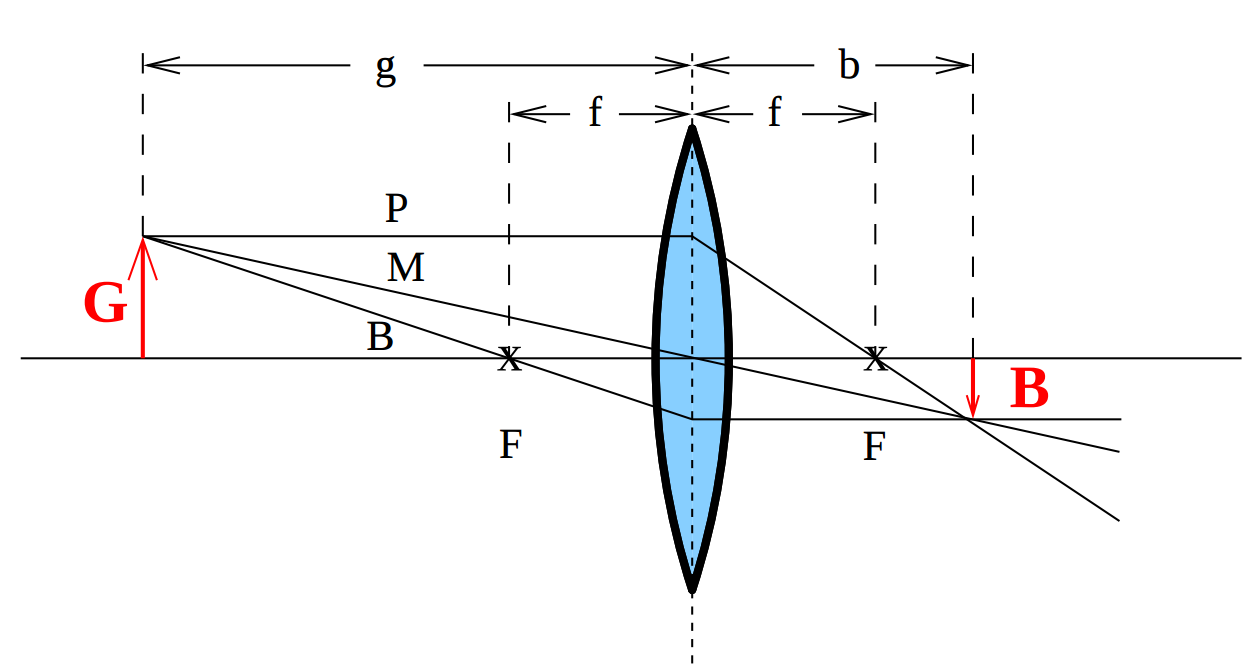
\includegraphics[width=1 \textwidth]{./pics/sammellinse.png}
    \caption{Sammellinse \cite{anleitung408}.}
    \label{fig: sammellinse}
  \end{subfigure}
  \begin{subfigure}{0.48\textwidth}
    \centering
    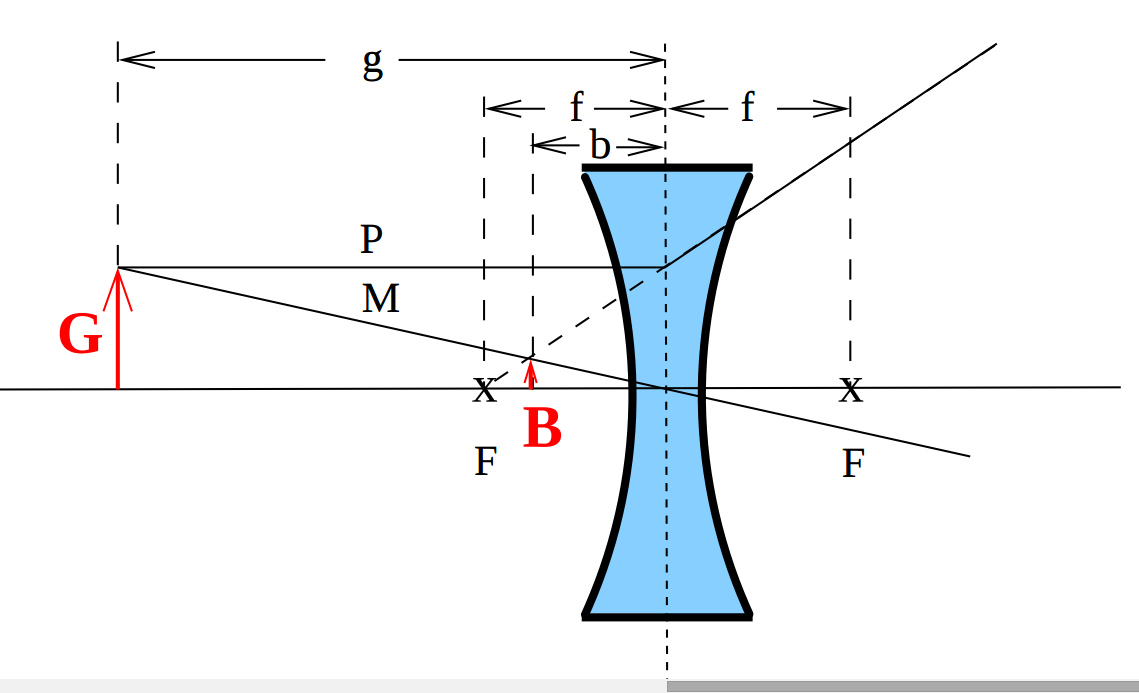
\includegraphics[width=1\textwidth]{./pics/zerstreungslinse.png}
    \caption{Zerstreuungslinse \cite{anleitung408}.}
    \label{fig: zerstreungslinse}
  \end{subfigure}
  \caption{Linsentypen}
  \label{fig: linsentypen}
\end{figure}
\begin{figure}
    \centering
    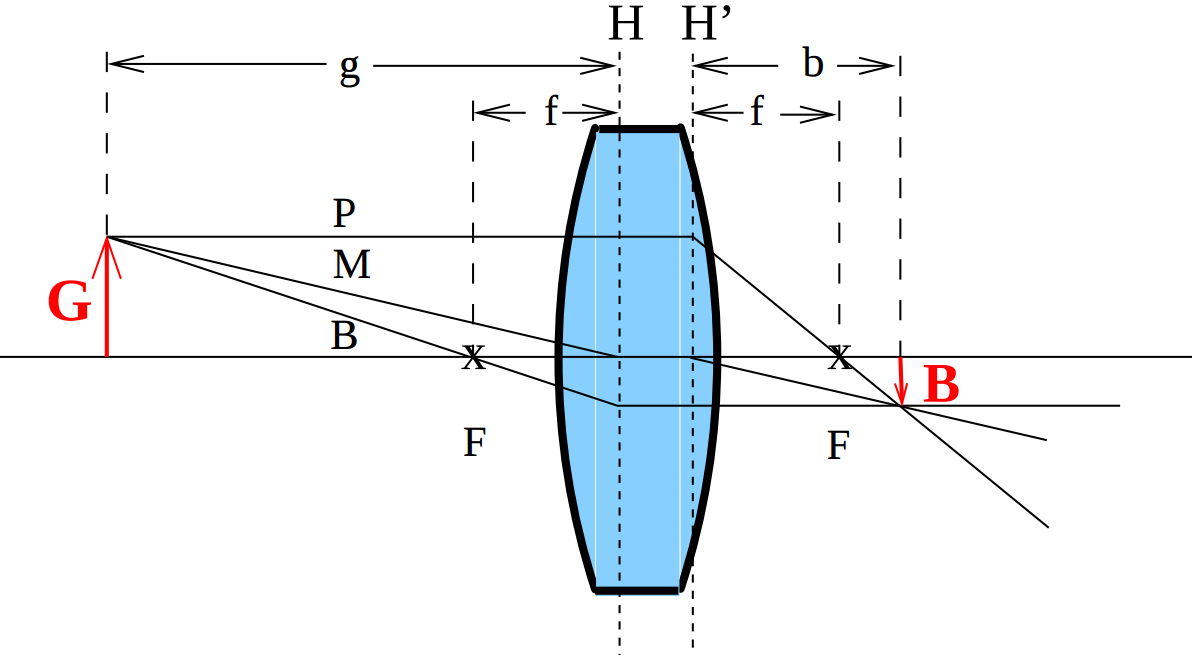
\includegraphics[width=0.6\textwidth]{./pics/dicke_linse.png}
    \caption{Dicke Linse \cite{anleitung408}.}
    \label{fig: dicke_linse}
\end{figure}

Um den Bildpunkt einer Linse zu konstruieren, werden drei Strahlen benötigt.
Zu diesen gehört der Parallelstrahl $P$, der Mittelpunktstrahl $M$ und der
Brennpunktstrahl $B$.
Der Parallelstrahl verläuft parallel zur optischen Achse und wird in der Hauptebene
zum Brennpunkt gebrochen. Der Mittelpunktstrahl verläuft vom Gegenstand mittig durch die
Linse. Zunächst läuft der Brennpunktstrahl durch den Brennpunkt der Linse, wird dann
an der Hauptebene gebrochen und verläuft dann parallel zur optischen Achse.
Aus der Bildkonstruktion erhält man das \emph{Abbildungsgesetz}
\begin{align}
  V_1&=\frac{B}{G} \label{eq: abbildungsgesetz_gross} \\
  V_2&=\frac{b}{g} \label{eq: abbildungsgesetz_klein}.
\end{align}
Hierbei beschreibt $V$ den Abbildungsmaßstab, $B$ die Bildgröße, $G$ die Gegenstandsgröße
und $g$ die Gegenstandsweite.

Aus Gleichung \eqref{eq: abbildungsgesetz} kann die Linsengleichung für dünne Linsen abgeleitet werden:
\begin{equation}
  \label{eq: linsengleichung}
  \frac{1}{f}= \frac{1}{b}+  \frac{1}{g} \qquad f= \frac{gb}{g+b}.
\end{equation}

Wie oben erwähnt verwendet man bei dicken Linse zwei Hauptebenen, um das Brechverhalten
zu beschreiben. Dieses Verfahren wir zusätzlich auch bei Linsensystem (vgl. Abbildung \ref{}) verwendet.
Um die Brennweite eines Linsensystems zu bestimmen, kann folgende Gleicung verwendet werden:
\begin{equation}
  \label{eq: gleichung_linsensystem}
  \frac{1}{f}=\frac{1}{f_1}+\frac{1}{f_2}-\frac{d}{f_1f_2}.
\end{equation}
Hierbei seien $f_1 \, \text{und} \, f_2$ die Brennweiten der beiden Linsen und $d$ der
Abstand der beiden Hauptebenen.
Die Bild-, Brenn- und Gegenstandsweite werden dann zur jeweiligen Hauptebene
bestimmt und sichern so die Gültigkeit der Linsengleichung.
Dennoch bietet das Hauptebensystem keine ideale Lösung, denn streng genommen
gilt es nur für achsennahe Strahlen. Bei achsenfernen Strahlen wird das Licht stärker
gebrochen und es können \emph{Abbildungsfehler}, z.\,B. nicht mehr scharfes Abbilden eines Bildes,
auftreten.

Eine weitere wichtige optische Größe ist die \emph{Brechkraft}
\begin{equation}
  \label{eq: brechkraft}
  D=\frac{1}{f}
\end{equation}
mit der Einheit Dioptrie $\map{dpt}=\si{\per \meter}$.
Bei einem Linsensystem, bestehend aus mehreren dünnen Linsen, erhält man die gesamte
Brechkraft $D\ua{G}$ mittels Summation der einzelnen Brechkräften
\begin{equation*}
  D\ua{G}=\sum_{i=1}^{N}D_i \qquad N\in\mathbb{N}.
\end{equation*}
